\section{Theory}

\subsection{Begriffe und Klassifikation}

\subsubsection{Ordnung}

Wie bei gewöhnlichen Differentialgleichungen ist die Ordnung
die höchste Ableitung der unbekannten Funktion, die in der
Differentialgleichung vorkommt.\\

\textbf{PDGL 1. Ordnung: } \qquad$F\biggl(x_1,\dots,x_n, u, \frac{\partial u}{\partial x_1},\dots,\frac{\partial u}{\partial x_n}\biggr)$

Sie kann durch Substitution $\frac{\partial u}{\partial x_i}\to p_i$ durch  $F(x_1,\dots,x_n,u,p_1,\dots,p_n),$
ausgedrückt werden.\\

\textbf{PDGL 2. Ordnung: } \qquad $F\biggl(x_1,\dots,x_n,u,
\frac{\partial u}{\partial x_1},\dots,\frac{\partial u}{\partial x_n},
\frac{\partial^2 u}{\partial x_1^2},\dots,\frac{\partial^2 u}{\partial x_n^2}\biggr)$

Sie kann durch Substitution $\frac{\partial u}{\partial x_i}\to p_i,~\frac{\partial^2 u}{\partial x_i\partial x_j}\to t_{ij}$ durch
$F(x_1,\dots,x_n,u,p_1,\dots,p_n,t_{11},t_{12},\dots,t_{n,n-1},t_{nn})$
ausgedrückt werden.

\subsubsection{Laplace-Operator}
\begin{tabular}{ll}
Kartesisch: $\Delta u(x,y,z)=\frac{\partial^2u}{\partial x^2}+\frac{\partial^2u}{\partial y^2}+\frac{\partial^2u}{\partial z^2}$
& Zylinder: $\Delta f ( \rho , \phi , z ) = \frac{1}{\rho} \frac{\partial}{\partial \rho}
\left( \rho\,\frac{\partial f}{\partial \rho} \right) +
\frac{1}{\rho^2}\frac{\partial^2 f}{\partial \phi^2} +
\frac{\partial^2 f}{\partial z^2}$ \\
Polar: $\Delta f(r, \phi ) =
\frac{\partial^2 f}{\partial r^2} +
\frac{1}{r}\frac{\partial f}{\partial r} +
\frac{1}{r^2}\frac{\partial^2 f}{\partial \phi^2}$
& Kugel: $\Delta f ( r , \vartheta , \phi ) = \frac{1}{r^2} 
\frac{\partial}{\partial r} \left( r^2  \,\frac{\partial f}{\partial r} \right) +
\frac{1}{r^2 \sin \vartheta}  \frac{\partial}{\partial \vartheta} \left(\sin\vartheta \, \frac{\partial f}{\partial \vartheta} \right) +
\frac{1}{r^2 \sin^2\vartheta}  \frac{\partial^2 f}{\partial \phi^2}$
\end{tabular}

\subsubsection{Umwandlung in System niedriger Ordnung}

\begin{tabular}{ll}
Gegeben:& $F\biggl(x,y,u,\frac{\partial u}{\partial x},\frac{\partial u}{\partial y},
\frac{\partial^2 u}{\partial x^2},\frac{\partial^2 u}{\partial x\partial y},
\frac{\partial^2u}{\partial y^2}\biggr)=0.$\\[0.2cm]
Substitution: & $p=\frac{\partial u}{\partial x},\qquad q=\frac{\partial u}{\partial y}$\\[0.2cm]
Für zweite Ableitungen: & $\frac{\partial^2 u}{\partial x^2}=\frac{\partial p}{\partial x},\quad \frac{\partial^2 u}{\partial x\partial y}=\frac{\partial p}{\partial y}=\frac{\partial q}{\partial x},\quad\frac{\partial^2 u}{\partial y^2}=\frac{\partial q}{\partial y}$\\[0.2cm]
Gleichungssystem 1.Ordnung& $p=\frac{\partial u}{\partial x},\quad q=\frac{\partial u}{\partial y},\quad\frac{\partial p}{\partial y}=\frac{\partial q}{\partial x}$
\end{tabular}

\subsubsection{Notationen einer PDGL, Gebiet $\Omega$}
\begin{minipage}{4cm}
	\begin{tabular}{ll}
	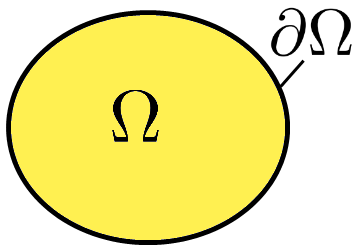
\includegraphics[width=3cm]{Content/Theory/Gebiet}&
	\end{tabular}
\end{minipage}
\begin{minipage}{4cm}	
	\begin{tabular}{ll}
		$\overset{\circ}{\Omega}$ & Innere Punkte\\
		$\partial\Omega$ & Rand\\
		$\overset{\_}{\Omega}$ & Gebiet $\Omega$ und Rand $\partial\Omega$\\
	\end{tabular}
\end{minipage}

Das Gebiet einer PDGL \textbf{muss} offen sein, nur dann ist die partielle Ableitung überall definiert. Das Gebiet ist offen, wenn um jeden Punkt im Gebiet $\Omega$ ein kleiner Ball gezeichnet werden kann, welches sich auch im Gebiet $\Omega$ befindet.

\textbf{Lösung einer PDGL:}\\
\begin{tabular}{ll}
Gegeben:& Gebiet $\Omega$, PDGL,Randwerte $\partial\Omega$\\
Lösung:& Funktion $u$: $\overset{\_}{\Omega}\rightarrow \mathbb{R}$, PDGL in $\Omega$ und Randwerte auf $\partial\Omega$\\
\end{tabular}

\subsubsection{Klassifikation einer PDGL}
\begin{tabular}{lll}
Ordnung:& \multicolumn{2}{l}{Höchste vorkommende partielle Ableitung}\\
Typ:& Linear: & Linear bei $u, x_1,...,x_n, \frac{\partial u}{\partial x_1},\ldots,\frac{\partial u}{\partial x_n}$\\
& Quasilinear: &  Linear bei $\frac{\partial u}{\partial x_1},\ldots,\frac{\partial u}{\partial x_n}$\\
& Nichtlineare: & Alles andere
\end{tabular}

\subsection{Charakteristiken}
\textbf{Wichtig:} Als Anfangsbedingungen dürfen \textbf{keine} Charakteristiken verwendet werden, sonst ist die Charakteristik die Lösung (anstatt Fläche ergibt sich eine Kurve).\\
\textbf{Wichtig:} Die Charakteristik darf den Rand nur einmal durchlaufen.\\
Nützlich für Qasilineare PDGL 1.Ordnung.\todo{Noch mehr?}\\
$$a(x,y,u)\cdot\partFrac{u}{x}+b(x,y,u)\cdot\partFrac{u}{y}=c(x,y,u) \qquad\Rightarrow\qquad a(x,y,u)\cdot\partFrac{u}{x}+b(x,y,u)\cdot\partFrac{u}{y}-c(x,y,u)=0$$\\


\begin{tabular}{ll}
Gebiet:& $\Omega{\ldots|x>0,alle y}$\qquad Randbedingung: $u(0,y_0)=g(y_0)$\\
Vektorielle schreibweise:& $\begin{bmatrix}
	a(x,y,u)\\ b(x,y,u)\\ c(x,y,u)
\end{bmatrix}\cdot 
\underset{\overrightarrow{n}~:~Normale ~auf~ Flaeche}{\underbrace{\begin{bmatrix}
\partFrac{u}{x} & \partFrac{u}{y} & -1
\end{bmatrix}}}=0$\\[1cm]
Tangenten:& $\overrightarrow{t}_x=\begin{bmatrix}1\\0\\ \partFrac{u}{x}\end{bmatrix}\qquad 
			\overrightarrow{t}_y=\begin{bmatrix}0\\1\\ \partFrac{u}{y}\end{bmatrix}$\\[1cm]
Lösungsweg& Für jeden Anfangspunkt $\begin{bmatrix} 0\\y_0\\g(y_0)\end{bmatrix}$ finde eine Charakteristik, diese nach $x$, $y$ auflösen.
\end{tabular}

Beispiel:\\
\begin{enumerate}
	\item PDGL mit Randbedingungen und Definitionsbereich: $\partFrac ux+2\partFrac uy=3$, \; $u(0,y)=g(y)=\sin(y) \Rightarrow u(0,y_0) = g(y_0) = \sin(y_0)$\\
	Therme in Matrixschreibweise: $\begin{bmatrix}a\\b\\c\end{bmatrix}=\begin{bmatrix}1\\2\\3\end{bmatrix}$
	\item Charakteristiken ausrechnen PDGL $\rightarrow$ DGL: 	$\frac {d}{dt}\begin{bmatrix}x(t)\\y(t)\\u(t)\end{bmatrix}=\begin{bmatrix}1\\2\\3\end{bmatrix}$
	\item DGL's lösen (für Standard-DGLS, siehe \ref{sec:dgls} auf Seite \pageref{sec:dgls}.): 
	$\begin{bmatrix}x\\y\\u\end{bmatrix}=\begin{bmatrix}t+x_0\\t+y_0\\t+u_0\end{bmatrix}$
	\item Anfangsbedingungen einsetzen: $\begin{bmatrix}x\\y\\u\end{bmatrix}=\begin{bmatrix}t+x_0\\t+y_0\\t+u_0\end{bmatrix}\Bigg|_{t=0}=
	\begin{bmatrix}x_0\\y_0\\u_0\end{bmatrix}=\begin{bmatrix}0\\y_0\\\sin(y_0)\end{bmatrix}$\\
	Lösung der DGL ist: $\begin{bmatrix}x\\y\\u\end{bmatrix}=\begin{bmatrix}1\\2\\3\end{bmatrix}\cdot t+ \begin{bmatrix}0\\y_0\\\sin(y_0)\end{bmatrix}$\\
	
	\item Eliminieren aller Variablen ausser $u,x,y$: $u=3x+\sin(y-2x)$
	\item Kontrolle
	Resultat ($u=3x+\sin(y-2x)$) ableiten und in Aufgabenstellung einsetzen $\partFrac ux+2\partFrac uy=3$ und schauen ob es erfüllt.
	
\end{enumerate}



\subsection{Methode Separation}
Wahl eines geeigneten Koordinatensystems ist wichtig.


\begin{enumerate}
\item \textbf{Ansatz} (Höchste Ableitung ausschlaggebend): 
	\begin{itemize}
		\item Für PDGL 1.Ordnung: $U(x,y)=X(x) + Y(y)$
		\item Für PDGL 2.Ordnung: $U(x,y)=X(x) \cdot Y(y)$ 
	\end{itemize}
\item \textbf{Einsetzen: } Ansatz in PDGL einsetzen.
\item \textbf{Separation: } Auf jeder Seite der PDGL darf nur noch eine Variable vorkommen. Die beiden jetzt gewöhnlichen DGL sind über eine Konstante gekoppelt (fixieren der Variable). Wahl der Konstante: Wenn Schwingung erwartet wird: $-k^2$, sonst $k$, ausser man weiss es besser ;-).
\item \textbf{Lösen der DGL's: } Man erhält eine Familie von Lösungen	
\item \textbf{Gesamtlösung "'Zusammenbasteln"': } (Linearkombination der Lösungen), Randbedingungen einhalten!
\end{enumerate}

\begin{minipage}{0.49\textwidth}
\textbf{Beispiel 1: } PDGL: $\frac1x\partFrac{u}{x}+\frac1y\partFrac{u}{y}=\frac{1}{y^2}$
\begin{enumerate}
	\item Ansatz:\\[0.4cm]
	$u(x,y)=X(x) + Y(y)$ (1.Ordnung)
	\item Einsetzen:\\[0.4cm]
	$\partFrac{u}{x}=X'(x)$\qquad $\partFrac{u}{y}=Y'(y)$ \quad $\Rightarrow$ \quad $\frac{X'(x)}{x}+\frac{Y'(y)}{y}=\frac{1}{y^2}$
	\item Separation:\\[0.4cm]
	$\frac{X'(x)}{x}=k=\frac{1}{y^2}-\frac{Y'(y)}{y}$
	\item DGL'2 lösen:\\[0.4cm]
	$X'(x)=k\cdot x \quad\Rightarrow\quad X(x)=\frac12 kx^2+C_x$\\
	$Y'(y)=\frac1y-ky \quad\Rightarrow\quad Y(y)=\ln(y)-\frac12 ky^2+C_y$
	\item Linearkombination:\\[0.4cm]
	$u(x,y)=\frac12 kx^2 - \frac12 ky^2+ln(y)+C$
\end{enumerate}

\textbf{Beispiel 2: } PDGL: $x^2\partFrac{^2u}{x^2}+x\partFrac{u}{x}+y^2\partFrac{^2u}{y^2}+y\partFrac{u}{y}=0$\\ 
Randbedingungen: $\Omega=[1,2]\times[1,2]$ \qquad $u=0$ auf $\partial\Omega$
\begin{enumerate}
	\item Ansatz:\\[0.4cm]
	$u(x,y)=X(x) \cdot Y(y)$ (2.Ordnung)
	\item Einsetzen:\\[0.4cm]
	$x^2X''(x)Y(y)+xX'(x)Y(y)+y^2X(x)Y''(y)+yX(x)Y'(y)=0$
	\item Separation: Division durch $X(x)Y(y)$\\[0.4cm]
	$\frac{x^2X''(x)}{X(x)}+\frac{xX'(x)}{X(x)}+\frac{y^2Y''(y)}{Y(y)}+\frac{yY'(y)}{Y(y)}=0\quad\Rightarrow\quad \frac{x^2X''(x)}{X(x)}+\frac{xX'(x)}{X(x)}=k=-\frac{y^2Y''(y)}{Y(y)}-\frac{yY'(y)}{Y(y)}$
	\item DGL'2 lösen:\\[0.4cm]
	$\frac{x^2X''(x)}{X(x)}+\frac{xX'(x)}{X(x)}=k\quad\Rightarrow\quad x^2X''(x)+xX'(x)-kX(x)=0$\qquad mit $X(1)=X(2)=0$\\
	$\frac{y^2Y''(y)}{Y(y)}-\frac{yY'(y)}{Y(y)}=-k\quad\Rightarrow\quad y^2Y''(y)+yY'(y)+kY(y)=0$\qquad mit $Y(1)=Y(2)=0$\\[0.4cm]
	Lösung der DGL hier nicht gemacht.
\end{enumerate}
\end{minipage}
\hfill
\begin{minipage}{0.49\textwidth}
\textbf{Beispiel 3: }PDGL: $\partFrac{^2u}{t^2}=\partFrac{^2u}{x^2}$ \quad $u(t=0,x)=0$\\
Randbedingungen: $x=[0,\pi]$ \\
\qquad\qquad $\partFrac{u}{t}(t=0,x)=\sin^3(x)=\frac34\sin(x)-\frac14\sin(3x)$
\begin{enumerate}
	\item Ansatz:\\[0.4cm]
	$u(t,x)=T(t) \cdot X(x) $ (2.Ordnung)
	\item Einsetzen:\\[0.4cm]
	$T''(t)\cdot X(x) = X''(x)\cdot T(t)$
	\item Separation:\\[0.4cm]
	$\frac{X''(x)}{X(x)}= -\mu^2=\frac{T''(t)}{T(t)}$
	\item DGL'2 lösen:\\[0.4cm]
		$X(x)=\sin(\mu x) \qquad T(t)=\sin(\mu t)$\\
		$X(x)=\cos(\mu x) \qquad T(t)=\cos(\mu t)$
	\item Linearkombination:\\[0.4cm]
		Die Randbedingungen $x=0$ und $x=\pi$ können nur mit $\sin(\mu x) $ und  positivem, ganzzahligen $\mu$ erfüllt werden. $cos(nx)$-Therme fallen weg.\\[0.4cm]
		$u(t,x)=\sum\limits_{n=1}^{\infty}{a_n\sin(nx)\sin(nt)} + \sum\limits_{n=1}^{\infty}{b_n\sin(nx)\cos(nt)}$\\[0.4cm]
		Die Koeffizienten $a_n$ und $b_n$ müssen mit Hilfe der Anfangsbedingungen zur Zeit $t=0$ bestimmt werden:\\[0.4cm]
		$u(0,x)=\sum\limits_{n=1}^{\infty}{b_n\sin(nx)}=0 \quad\Rightarrow\quad b_n=0$\\[0.2cm]
		$\partFrac{u}{t}(\pi,x)=\sum\limits_{n=1}^{\infty}{a_nn\sin(nx)}=\sin^3(x)=\frac34\sin(x)-\frac14\sin(3x) \quad\Rightarrow\quad a_1=\frac34 \quad a_3=-\frac{1}{12}\quad a_k=0$ für $k\neq 1,3$\\[0.4cm]
		$u(t,x)=\frac34\sin(x)\sin(t)-\frac1{12}\sin(3x)\sin(3t)$
\end{enumerate}
\end{minipage}





\subsection{Transformationen}
\todo{Beschreibung}


\begin{itemize}
\item Der Übergang von Funktionen zu Fourierreihen verwandelt eine partielle
Differentialgleichung in eine Familie gewöhnlicher Differentialgleichungen für
die einzelnen Fourier-Koeffizienten.
\item Integraltransformationen können ein partielle Differentialgleichung in eine
Familie partieller Differentialgleichungen mit weniger Variablen oder sogar
gewöhnlicher Differentialgleichungen verwandeln.
\item Integraltransformationen und die Rücktransformationen können Formeln
für die Lösungen gewisser partieller Differentialgleichungen liefern, und
damit die Frage beantworten, für welche Randwertvorgaben die Gleichungen
gut gestellt sind.
\end{itemize}

\subsubsection{Fourierreihe}

$\boxed{u(t,x)=\frac{a_0(t)}{2}+\sum\limits_{k=1}^{\infty}{a_k(t)\cos(kx)+b_k(t)\sin(kx)}}$\\[0.4cm]

\textbf{Beispiel:} Schwingende Saite: $\boxed{\partial_t^2u=\partial_x^2u}$\\

\begin{itemize}
\item Ansatz der Fourieranalyse in PDGL einsetzen:
$\partial_t^2(t,x)=\frac{a_0''(t)}{2}+\sum\limits_{k=1}^{\infty}{a_k''(t)\cos(kx)+b_k''(t)\sin(kx)}$\\
$\partial_x^2(t,x)=-\sum\limits_{k=1}^{\infty}{a_k(t)k^2\cos(kx)+b_k(t)k^2\sin(kx)}$\\
$\partial_t^2(t,x)=\frac{a_0''(t)}{2}+\sum\limits_{k=1}^{\infty}{a_k''(t)\cos(kx)+b_k''(t)\sin(kx)}=-\sum\limits_{k=1}^{\infty}{a_k(t)k^2\cos(kx)+b_k(t)k^2\sin(kx)}=\partial_x^2(t,x)$\\[0.2cm]
$\boxed{\Rightarrow\quad \frac{a_0''(t)}{2}+\sum\limits_{k=1}^{\infty}{\big(a_k''(t)+a_k(t)k^2\big)\cos(kx)+\big(b_k''(t)+b_k(t)k^2\big)\sin(kx)}=0}$
\item Diese Gleichung ist nur Lösbar wenn alle Koeffizienten verschwinden (Fourier-Theorie):\\[0.2cm]
$a_0''(t)=0 \qquad a_k''(t)=-k^2a_k(t)\qquad b_k''(t)=-k^2b_k(t)$
\item Durch die Fouriertransformation wurde die PDGL in ein DGL-System überführt, die Lösungen sind wohlbekannt:\\[0.2cm]
$a_0(t)=m_0(t)+c_0\qquad a_k(t)=A_k^a\cos(kt)+B_k^a\sin(kt)\qquad b_k(t)=A_k^b\cos(kt)+B_k^b\sin(kt)$
\end{itemize}


\subsubsection{Anfangsbedingungen}
Die Differentialgleichungen für die Koeffizienten ak(t) und bk(t) können erst dann
vollständig gelöst werden, wenn Anfangs oder Randbedingungen gegeben sind.\\
\begin{itemize}
\item Anfangsbedingungen für Wellengleichung:\\
\quad $u(0,x)=f(x)\qquad \partFrac{u}{t}=g(x)$
\item Die Funktionen f und g können auch als Fourrierreihe dargestellt werden:\\
$f(x)=\frac{a_0^f}{2}+\sum\limits_{k=1}^{\infty}{a^f_k\cos(kx)+b^f_k\sin(kx)}$\\[0.2cm]
$g(x)=\frac{a_0^g}{2}+\sum\limits_{k=1}^{\infty}{a^g_k\cos(kx)+b^g_k\sin(kx)}$
\item Zusammen mit dem Ansatz für $u(t,x)$ ergeben sich die Gleichungen (für $t=0$):\\
$\frac{a_0(0)}{2}+\sum\limits_{k=1}^{\infty}{a_k(0)\cos(kx)+b_k(0)\sin(kx)}=\frac{a_0^f}{2}+\sum\limits_{k=1}^{\infty}{a_k^f\cos(kx)+b^f_k\sin(kx)}$\\[0.2cm]
$\frac{a'_0(0)}{2}+\sum\limits_{k=1}^{\infty}{a_k'(0)\cos(kx)+b_k'(0)\sin(kx)}=\frac{a_0^g}{2}+\sum\limits_{k=1}^{\infty}{a_k^g\cos(kx)+b^g_k\sin(kx)}$
\item Koeffizientenvergleich ergibt:\\
$a_k(0)=a_k^f\qquad a_k'(0)=a_k^g\qquad b_k(0)=b_k^f\qquad b_k'(0)=b_k^g$
\item Die vollständige Lösung ist damit:\\
$u(t,x)=\frac{a_0^g(t)+a_0^f}2+\sum\limits_{k=1}^{\infty}{\left(a_k^f\cos(kt)+\frac 1k a_k^2\sin(kt)\right)\cos(kx)+\left(b_k^f\cos(kt)+\frac 1k b_k^2\sin(kt)\right)}\sin(kx)$
\end{itemize}

\subsubsection{Inhomogene Wellengleichung}

Das Verfahren lässt sich auch auf die inhomogene Wellengleichung verallgemeinern. Das Störglied wird dabei ebenfalls als Fourierreihe entwickelt.

$\partial_t^2u-\partial_x^2u=f \qquad \Rightarrow \qquad f(t,x)=\frac{a_0^f(t)}{2}+\sum\limits_{k=1}^{\infty}{a^f_k(t)\cos(kx)+b^f_k\sin(kx)}$



\subsubsection{Laplace-Transformation}

$\boxed{F(t)=\int\limits_{0}^{\infty}{f(t)\e^{-st}} dt}$ \qquad Siehe auch weiter hinten in der Zusammenfassung!\\

\textbf{Lösung einer ODGL:}\\

$\dot{x}(t)+p x(t)=f(t) \qquad f(t)=q$\\
$\dot{x}(t)+p x(t)=f(t)\FT s X(s)-x(0)+pX(s)=F(s) \qquad f(t)\FT F(s)=\frac{q}{s}$\\

$\Rightarrow X(s)=\frac{F(s)+x(0)}{s+p}=\frac{q+x(0)}{s(s+p)}\Big|_{x(0)=0}\IFT x(t)=\frac{q}{p}(1-\e^{-pt})$\\

\textbf{Lösung einer PDGL:}\\

$\partFrac{u}{t}+x\partFrac{u}{x}=x\qquad t\geq 0,\quad x\geq 0\qquad u(x,0)=0,\quad u(0,t)=0\qquad x,t>0$\\

Transformation: $\partFrac{u}{t}+x\partFrac{u}{x}=x\FT sU(s,x)-u(x,0)+x\partFrac{U(s,x)}{x}=\frac{x}{s}\qquad \Rightarrow \qquad U(s,x)=\frac{x}{s(s+1)}$\\
$U(s,x)\IFT x(1-\e^{-t})$












\subsection{PDGL 2.Ordnung}
Lineare partielle Differentialgleichungen zweiter Ordnung haben die Form:
$\boxed{\sum\limits_{i,j=1}^{n}{a_{ij}\partial_i\partial_j u}+\sum\limits_{i=1}^{n}{b_i\partial_i u}+cu=f}$

\subsubsection{Klassifikation}
Klassifikation nur für PDEs zweiter Ordnung!

\begin{minipage}{9cm}
  Eigenwertberechnung: (z.B. von $ \partial^2_xu+2\partial_x\partial_yu+\partial^2_yu=0 $) 
  \begin{enumerate}
    \item Symmetrische Matrix aufstellen und $\lambda$ in der Diagonalen abziehen. Z.B.: $A = \begin{pmatrix}
      \partial_x^2 & \partial_x \partial_y \\
      \partial_y \partial_x  & \partial_y^2
    \end{pmatrix}$\\
    Bei diagonalen Matrizen entsprechen die Eigenwerte den Diagonaleinträgen.
    \item Determinante gleich 0 setzen: $\det(\mathbf{A}-\lambda \mathbf{I}) = 0\quad\Rightarrow\quad \lambda_i$
    \item Gleichung lösen
  \end{enumerate}
\end{minipage}
\begin{minipage}{9cm}
  Alternativ (wenn z.B. sehr wüste PDE klassifiziert werden muss), können auch via Spur und Determinante die Vorzeichen der Eigenwerte herausgefunden werden:
  \begin{enumerate}
    \item Siehe links (Eigenwertberechnung): Matrix $A$ aufstellen
    \item Determinante berechnen und versuchen aus Tabelle zu lesen:
     $\det A = a_{00}a_{11} - a_{12}a_{21} = \lambda_1 \lambda_2$
    \item Spur berechnen und versuchen aus Tabelle zu lesen:
      $\tr(A) = a_{00} + a_{11} = \lambda_1 + \lambda_2$
  \end{enumerate}
  
\end{minipage}

\begin{tabular}{|l||l|l|l|l|}
\hline
\multirow{2}{*}{Klasse}&\multicolumn{3}{|c|}{Anzahl Eigenwerte}&\multirow{2}{*}{Beispiel}\\
&Positiv&Negativ&Verschwindend&\\
\hline
hyperbolisch& n-1 & 1 & 0 & Wellengleichung\\
\hline
parabolisch& n-1 & 0 & 1 & Wärmeleitung\\
\hline
elliptisch&	n & 0 & 0 & Potential\\
\hline
ultrahyperbolisch & >1 & >1 & 0 & -\\
\hline
\end{tabular}

\subsection{Elliptische PDGL}
$\Delta u=f\qquad \omega=\{(x,y)|y\geq 0\},\quad u(x,y)=ay$

\textbf{Satz:} Wenn $\Omega$ beschränkt und zusammenhängend, dann ist die Lösung u immer eindeutig.\\

\textbf{Beweis:} Annahme: $u=u_1-u_2$\\
Einsetzen: $\Delta u_1 - \Delta u_2=f-f=0$\\
$\left.(u_1-u_2)\right|_{\partial \omega}=g-g=0$\\
$\Delta u=0 \qquad \left.u\right|_{\partial\Omega}=0$\\
Falls $u=0$ eine Lösung, dann gibt es nur eine Lösung.

\subsubsection{Maximumprinzip} 

Wenn gilt $\Delta u=0$, dann befinden sich die Extrema (Maxima und Minima der Funktion) auf dem Rand $\partial\Omega$.

\subsubsection{Beispiel (Übungslösungen)}
Eine elliptische PDGL wie $\Delta u = c$ hat mit der vorgegebenen
Dirichlet-Randwerten nur eine Lösung. Zur Erinnerung: Der Grund war das
Maximum-Prinzip. Gäbe es nämlich eine zweite Lösung $\bar v(r,\phi)$ mit
gleichen Randwerten, wäre $v - \bar v$ eine Lösung der Gleichung $\Delta (v -
\bar v) = 0$ also harmonische Funktion. Die Randwerte von $v - \bar v$ sind 0. Da eine
harmonische Funktion das Maximum auf dem Rand annimmt ist $v - \bar v = 0$ die
Lösung ist also eindeutig.

\newpage
\subsubsection{Greensche Funktion} 

Eine elliptische PDGL wird mittels Inversion von $\Delta$ gelöst. Dieser Umkehr geschieht mittels Greenscher Funktion, welche die Umkehrfunktion $\Delta$ ist\qquad $\Delta$: Laplace-Operator.

$u(x)=\int\limits_\Omega{\sigma(x,\xi)f(\xi)d\xi}+\int\limits_\Omega{h(x,\xi)f(\xi)d\xi}\qquad \sigma(x,\xi)=
\begin{cases}
	\frac 12|x-\xi| & n=1\\ 
	\frac 1{2\pi}\log|x-\xi| & n=2\\
	-\frac 1{4\pi}\frac{1}{|x-\xi|} & n=3\\
	\frac {1}{(2-n)\mu(S^{n-1})}|x-\xi|^{2-n} & n\geq 3\\
\end{cases}$\\


Greensche Funktion: $G(x,\xi)=\sigma(x,\xi)+h(x,\xi)$

Satz: Ist $\Omega$ ein Gebiet, auf dem das Dirichlet Problem eindeutig lösbar ist, dann gibt es eine Funktion $G(x,\xi)$, welche als Funktion von x die Gleichung

$\Delta G(x,\xi)=\delta(x-\xi)$

löst mit homogenen Randbedingungen.
Lösung: $u(x)=\int\limits_{\Omega}^{}{G(x,\xi)f(\xi)d\xi}+\int\limits_{\partial\Omega}g(\xi)\cdot\grad{\xi}G(x,\xi)d\eta\qquad \eta:\text{ Normale von }\partial G$

\subsubsection{Mittelwerteigenschaft harmonischer Funktionen}

$\Delta h=0$\qquad Mittelwerteigenschaft:\qquad $h(x)=
\begin{cases}
	\frac{h(x+\delta)+h(x-\delta)}{2}& n=1 \\ 
	\frac 1{2\pi r} \int\limits_{S_r^1}{h(x+\xi)d\xi} & n=2\\
	\frac 1{4\pi r^2} \int\limits_{S_r^2}{h(x+\xi)d\xi} & n=3\\
\end{cases}$
%\subsection{Parabolische PDGL}
\todo{Beschreibung}
\subsection{Hyperbolische PDGL}
\todo{Beschreibung}


